\newcommand{\tax}{\textsf{t\_ax}}
\newcommand{\tpi}{\textsf{t\_pi}~}
\newcommand{\tlam}{\textsf{t\_lam}~}
\newcommand{\tapp}{\textsf{t\_app}~}
\newcommand{\ptc}{\textsf{p\_tc}}

\newcommand{\rall}{\textsf{r\_all}}
\newcommand{\rarr}{\textsf{r\_arr}}
\newcommand{\rapp}{\textsf{r\_app}}
\newcommand{\rtapp}{\textsf{r\_App}}
\newcommand{\rlam}{\textsf{r\_lam}}
\newcommand{\rtlam}{\textsf{r\_Lam}}

\newcommand{\D}{\mathcal{D}}

While the HOAS approach is quite elegant in general,  manual manipulation of contextual information, as is necessary in Abella, can be cumbersome and annoying. 
The need for copious amounts of inversion lemmas that mostly deal with the fact that contexts can a priori contain arbitrary judgements was particularly irritating.
An alternative is the programming and proof environment Beluga \cite{Pientka:IJCAR10,Pientka:FLOPS10,Pientka:CADE15} where we can encode formal systems within the logical framewwork LF \cite{Harper93jacm} using HOAS and then reason about them by writing total programs that analyze derivation trees using pattern matching. 
In Beluga we do not simply deal with objects (like types, terms, typing derivations), but with contextual objects where we pair an object together with the context in which it is meaningful\cite{Nanevski:ICML05,Pientka:POPL08}.
Contexts describe all the free variables that occur in a given object and are first-class. 
% Context invariants can be described and checked by context schema checking

So both Abella and Beluga delegate object level-binding to meta-level binding, but while Abella then proceeds to utilise global nominal constants, Beluga instead employs local contexts and contextual objects. 
The difference is best illustrated with an example.
Consider, in Abella, the F-function type $n_1 \to n_2$ where $n_1$ and $n_2$ are global nominal constants. 
It is relatively easy to prove that $\{\emptyctx \vdash \istyFh{n_1 \to n_2}\}$ entails absurdity.
In other words, there exist types $A \OF \TyF$, that are not well-formed.
To be precise, well-formedness checks that a type does not have dangling variables (this is the reason we have made the empty context explicit).
%
\newcommand{\bc}[2]{\ensuremath{[\,#1\,\vdash #2\,]}}
In Beluga on the other hand, this example cannot even be expressed, as \[\bc{\emptyctx}{x \to y} \OF \bc{\emptyctx}{\TyF}\] is not meaningful in Beluga's type theory. The local variables $x$ and $y$ must be declared in the context on the left hand side of $\vdash$ and hence Beluga will simply raise an error that $x$ and $y$ are free. This happens even before type checking. Also observe how the type itself is a contextual object. An immediate consequence of this is that the concept of a F type formation judgement does not even make sense in Beluga, which will have an impact on the representation of our equivalences.

The definition of our object languages in Beluga is almost identical to the one in Abella.
The only difference is that term abstraction and type application rules of the F type system do not request the respective types are well-formed, as this is immediate for the above reasons.
Hence we won't repeat the formal definitions and instead focus on Beluga's treatment of contextual information.

In contrast to Coq, where contexts are modelled explicitly and are located conceptually on the same level as object language terms and types, and Abella, where the implicit object level reasoning context appears as an explicit list of arbitrary judgements at the reasoning level, Beluga contexts are special reasoning level first class objects that can exhibit rather complex structures.
%
This is achieved through a separate typing mechanism that ascribes \emph{context schemas} to meta-level variables that represent contexts.
In Beluga, a context is a structured ordered sequence of declarations where each declaration can depend on prior declarations and encapsulate multiple pieces of related information using a dependent record, i.e.~not only do we have dependency structures within each record but also possibly between multiple records.
% A context schema is then a set of admissible $\Sigma$-types for such a list of records.
In particular, this entails that contexts need not be homogeneous.  
As a simple example consider the following schema, which is used to prove propagation for \SysL.
\begin{align*}
  S_{\lambda W} \eqdef [x\of\TmL \mrel{;} \typingLh{x}{\Prp}] \mrel{+} [x\of\TmL \mrel{;} \typingLh{x}{a} \mrel{;} \typingLh{a}{\Prp}]
\end{align*}
This schema already separates PTS variables that are used as types (i.e. those from records matching the left variant) and those used as terms (i.e. those from records matching the variant on the right).
Recall that this is a semantic distinction, i.e.~syntactically there is only a single sort.

Let us next consider the proof of \SysL propagation in Beluga, which can be done from first principles and surprisingly is the only language-local meta-theoretic result required to complete the challenge.
We use this to illustrate how a simple inductive Beluga proof is constructed.
The first hurdle we have to overcome is the absence of disjunction and existential quantification in Beluga's meta logic.
This is achieved by simply defining a predicate $\mathsf{type\_correct}\,a$ as follows:
%\begin{align*}
%  \mathsf{type\_correct}\,a \iff a = \Typ \mOr \mEx{u} \typingLh{a}{u} \mAnd \sortLh{u}
%\end{align*}
\[
\begin{array}{c}
% \fbox{\textsf{type\_correct}~a}~~Type $a$ 
\inferrule*[right=p\_tc$_1$]{~}{\mathsf{type\_correct}~\Typ} \qquad
\inferrule*[right=p\_tc$_2$]{ \typingLh{a}{u} \quad \sortLh{u}}{\mathsf{type\_correct}~a}
\end{array}
\]
Since Beluga is not equipped with a tactic language, we prove propagation by implementing a total recursive function of the following type:
\begin{align*}
  \mAll{\Gamma \of S_{\lambda W}} \bc{\Gamma}{\typingLh{A}{B}} \implies \bc{\Gamma}{\mathsf{type\_correct}\,B}
\end{align*}
The proof proceeds by induction on $d \OF \bc{\Gamma}{\typingLh{A}{B}}$. There are 7 cases to consider, 3 of which are variable cases that arise from the context schema (see \cite{Pientka:TLCA15} for a description of coverage for contextual objects and contexts).
Let us first look at the cases that arise from the four rules (\tax, \tpi, \tlam, \tapp)~defining ${\typingLh{A}{B}}$ in Fig.~\ref{fig:sys-l-abella}.
 
When $d$ is a derivation $\bc{\Gamma}{\tax}$ of $\bc{\Gamma}{\typingLh{\Prp}{\Typ}}$, then $\bc{\Gamma}{\mathsf{type\_correct}\,\Typ}$ clearly holds using \ptc$_1$ as a witness.
When $d$ is a derivation ending in \tpi~rule, 
 $\bc{\Gamma}{\mathsf{type\_correct}\,\Prp}$ is easily established using \ptc$_2$ the axioms from Fig.~\ref{fig:sys-l-abella}. For the case where $d$ ends in the abstraction rule \tlam~we have to show that $\bc{\Gamma}{\typingLh{\Prod{A}B}{\Prp}}$ holds, and thus $\bc{\Gamma}{\mathsf{type\_correct}\,\Prod{A}B}$, which is easy.

The interesting case is application where we have $d = \bc{\Gamma}{\tapp\,\D_{AB}\,\D_{A}}$ and stands for $\bc{\Gamma}{\typingLh{M\,N}{\lpApp{B}{N}}}$, where $\D_{AB}$ is a sub-derivation for $\bc{\Gamma}{\typingLh{M}{\Prod{A}B}}$ and $\D_{A}$ stands for a sub-deriation $\bc{\Gamma}{\typingLh{N}{A}}$.
Applying our inductive hypothesis to $\bc{\Gamma}{\D_{AB}}$ yields a derivation for $ \bc{\Gamma}{\mathsf{type\_correct}\,\Prod{A}B}$. Using pattern matching, we determine there is only one possible way we could construct a derivation of this type, namely using $\bc{\Gamma}{\mbox{\ptc}_2~\D~\D_u}$, since  $\Prod{A}B \neq \Typ$. Hence, we know that there is a sub-derivation $\D$ ending in 
$\bc{\Gamma}{\typingLh{\Prod{A}B}{u}}$ and a derivation $\D_u$ standing for $\bc{\Gamma}{\sortLh{u}}$


%By inversion on the definition of $\mathsf{type\_correct}$ using \textsc{p\_tc2}, we have two sub-deriations: $\D_P$ stands for know $\bc{\Gamma}{\Prod{A}B}} $
% $\bc{\Gamma}{p_{\mathsf{tc2}}\,d_P\,d_u} \OF

Further pattern matching on $\D_P$ using the \tpi~rule, 
reveals a derivation $\D_B$ for $\typingLh{\lpApp{B}{x}}{\Prp}$ in the extended context $\Gamma, x\of\TmL, \typingLh{x}{A}$. 
% $\bc{\Gamma, [x \of\TmL \mrel{;} \typingLh{x}{A}]}{\typingLh{\lpApp{B}{x}}{\Prp}}$
%
Substitutivity is natively provided in Beluga, so we have $\lpApp{\D_B}{N,d_A} \OF \bc{\Gamma}{\typingLh{\lpApp{B}{N}}{\Prp}}$ and can close the case.

This brings us to variable cases where we extract a variable from the context. 
Recall the context schema definition of $S_{\lambda W}$.
The left alternative has one occurrence of a typing assumption, while the right alternative has two.
Two of these fix $B = \Prp$ so the requisite universe containing $B$ is simply $\Typ$.
If however we happen to have extracted the first typing assumption from a record of the right variant, then $S_{\lambda W}$ tells us that the second typing assumption from the very same block assigns $B$ the type $\Prp$, which is the required universe to close the case.
%
The most interesting part here was the use of substitutivity, which in Coq required a significant amount of boilerplate development.
In Abella we first had to obtain substitutivity of PTS typing as a special case of a cut theorem and combine this with the aforementioned context inversion Lemmas.

At this point we can tackle the actual solution to our challenge.
Both $\tyr$ and $\tmr$ are again encoded as LF types at the same level where the object languages are defined. The definitions are exactly identical to those in Abella.
Since Beluga does not natively provide equality, we also define three LF types that encode equality of the various syntactic sorts, each with a single reflexive constructor.

We begin with the functionality of $\tyr$, that is, we implement a recursive function of type
\begin{align*}
  \mAll{\Gamma \of S_{\tyr}} \bc{\Gamma}{A \tyr a} \implies \bc{\Gamma}{A \tyr a'} \implies \bc{\Gamma}{a =_{\lambda} a'},
\end{align*}
where 
\begin{align*}
  S_{\tyr} \eqdef [y \of \TmL] \mrel{+} [x\of\TyF \mrel{;} y\of\TmL \mrel{;} h\of x \tyr y]
\end{align*}
The context schema expresses the tightest invariant that holds about the rules defining the $\tyr$ relation.% on page \pageref{rel-rules}.
In particular, we may either introduce a $\TmL$ variable in the rule \rarr~or we introduce a $\TyF$ variable $x$ and a $\TmL$ variable $y$ together with $x \tyr y$ in the rule \rall.

We go over the definition of this function in detail to illustrate how contextual information is generated and processed when binders are traversed.
At a high level, the proof is by induction on the derivation of $d_1 \OF \bc{\Gamma}{A \tyr a}$ and pattern matching on $d_2 \OF \bc{\Gamma}{A \tyr a'}$.
We have to cover three cases, two structural and one for a context extraction.

Let $d_1$ be a derivation that ends in the rule \rarr, i.e.~ is $A = B \to C$ and $a = \Prod{b}c$ for some $B,C,b,c$. Then $d_1 = \bc{\Gamma}{\rarr~\D_{11}~\D_{12}}$ where 
we have sub-derivations $\D_{11} \OF \bc{\Gamma}{B \tyr b}$ and $\D_{12} \OF \bc{\Gamma, y \of \TmL}{C \tyr \lpApp{c}{y}}$.
As a consequence, $d_2$ must have also ended with the \rarr~rule. This is accomplished by pattern matching on $d_2 = \bc{\Gamma}{\rarr~\D_{21}~\D_{22}}$. Hence $a' = \Prod{b'}c'$, with sub-derivations $\D_{21} \OF \bc{\Gamma}{B \tyr b'}$ and $\D_{22} \OF \bc{\Gamma, [y \of \TmL]}{C \tyr \lpApp{c'}{y}}$.
We have to prove that $\Prod{b}c =_{\lambda} \Prod{b'}c'$, which is only possible if we can unify $b$ with $b'$ and $c$ with $c'$.
This is easily achieved through invocations of the inductive hypothesis on $\bc{\Gamma}{\D_{11}}$ and $\bc{\Gamma}{\D_{21}}$ and, respectively, on $\bc{\Gamma}{\D_{12}}$ and $\bc{\Gamma}{\D_{22}}$.

Next we consider the \rall~rule. By pattern matching on $d_1$ with $\bc{\Gamma}{\rall~\lambda x.\lambda u.\D_1}$ we obtain $A = \All B$, $a = \Prod{\Prp} b$, 
and $\D_1$ stands for $\bc{\Gamma, x \of \TyF, y \of \TmL, h \of x \tyr y}{\lpApp{B}{x} \tyr \lpApp{b}{y}}$.  
Similarly, by pattern matching on $d_2$ with $\bc{\Gamma}{\rall~\lambda x.\lambda u.\D_2}$ we learn $a' = \Prod{\Prp} b'$ and $\D_2$ stands for 
$\bc{\Gamma, x \of \TyF, y \of \TmL, h \of x \tyr y}{\lpApp{B}{x} \tyr \lpApp{b'}{y}}$.  
%
To apply the induction hypothesis, we also must ensure that the context invariant is satisfied. We hence pack the assumptions $ x \of \TyF, y \of \TmL, h \of x \tyr y$ in a dependent record $r$ and 
invoke the induction hypothesis on $\bc{\Gamma, r}{\lpApp{\D_1}{r_x,r_y,r_h}}$ and $\bc{\Gamma, r}{\lpApp{\D_2}{r_x,r_y,r_h}}$. We rely on the built-in simultaneous substitution operation to replace $x$ with the projection $r_x$, $y$ with the projection $r_y$, and $h$ with the projection $r_h$. By uncurrying the LF functions denoting parametric and hypothetical derivations, we can enforce the stated context invariant which guarantees naturally that whenever we have a $\TyF$ variable $x$, we also must have a related  $\TmL$ variable $y$ (and vice versa).
 
% The scenario is similar for $d_{21}$.
% That is, we cannot directly apply our inductive hypothesis to unify $b$ and $b'$.


Finally, we consider the variable case where we extract a declaration from the context. The derivation $d_1$ must have come from a block of the form $r \OF [x\of\TyF \mrel{;} y\of\TmL \mrel{;} h \of x \tyr y]$, that is $d_1 = r_h$ and stands for a derivation
$\bc{\Gamma}{r_x \tyr r_y}$. Note that by assumption $d_2$ stands for $\bc{\Gamma}{r_x \tyr a'}$.  By pattern matching on $d_2$, $a'$ must be $r_y$, since assumptions in a context are unique.
We can use $S_{\tyr}$ to obtain injectivity of $\tyr$ in a similar fashion.
%
In contrast, to context relations that are commonly used in Abella and Coq, Beluga supports developing proofs by enforcing context invariants using context schemas. While in this example, we can directly derive the context invariant needed in the proof from the definitions of $\tyr$ and $\tmr$, this may not always be the case.  Instead, we may need to generalize. The contrast between the joint context in Beluga versus the relational context approach in Abella is also highlighted in \cite{Felty:ITP10,Felty:orbi-survey}.


To obtain functionality and injectivity of $\tmr$ we can follow a similar pattern, generalizing the previous context schema  to 
\begin{align*}
  S_{\tmr} \eqdef [x\of\TmF \mrel{;} y\of\TmL \mrel{;} h\of x \tmr y] \mrel{+} [x\of\TyF \mrel{;} y\of\TmL \mrel{;} h\of x \tyr y]
\end{align*}
Again this schema can be derived from the definition of the $\tmr$ rules. 
When we compare the two context schemas it should quickly be come apparent that any $\Gamma \of S_{\tmr}$ contains at least as much information as required by $S_{\tyr}$. We also note that while the rules $\tyr$ do only refer to $\tyr$ assumptions and not to $\tmr$ assumptions. Based on this dependency \cite{Virga99phd}, Beluga supports strengthening. In other words, if we need to appeal to functionality and injectivity of $\tyr$ within the proof of functionality and infjectivity of $\tmr$, we may strengthen the given context such that it satisfies $S_{\tyr}$, appeal to functionality and injectivity of $\tyr$, and the weaken the result to use it in the context satisfying $S_{\tmr}$ (see \cite{Felty:orbi-survey} for a detailled discussion especially in contrast to context relations).

% Beluga is capable of implicitly strengthening contexts in this way.
% So when the proof of functionality of $\tmr$ relies on the functionality of $\tyr$ we can directly pass the given complex context and do not need to invoke any stripping functions or strengthening lemmas beforehand.
% In other words, we get directly $\Gamma \of S_{\tyr}$ rather than $\mathsf{str}(\Gamma) \of S_{\tyr}$.
% The only other interesting aspect here than is the injectivity of $\tmr$ relies on $\tyr$ and $\tmr$ having disjoint ranges, which thanks to higher-order unification is very easy to obtain under contexts $\Gamma \of S_{\tmr}$.

When it comes to the totality and preservation results we define a predicate $\mathsf{exists\_rel\_prop}~A$ that succeeds, if there exists a type $A$ s.t. $A \tyr a$ and $\typingLh{a}{\Prp}$: 
\begin{align*}
\inferrule*{A \tyr a \quad \typingLh{a}{\Prp}}{ \mathsf{exists\_rel\_prop}\,A}
%  \mathsf{exists\_rel\_prop}\,A \iff \mEx{a} A \tyr a \mAnd \typingLh{a}{\Prp}
\end{align*}
The result itself is then established with a function of type
\begin{align*}
  \mAll{\Gamma \of S_{\tyr W}^{\rightarrow}} \mAll{A \of \bc{\Gamma}{\TyF}} \bc{\Gamma}{\mathsf{exists\_rel\_prop}\,A}
\end{align*}
where $S_{\tyr W}$ extends the context schema $S_{\tyr}$ with additional typing information in each block:
\begin{align*}
  S_{\tyr W}^{\rightarrow} \eqdef [y\of\TmL \mrel{;} v\of\typingLh{y}{a}] \mrel{+} [x\of\TyF \mrel{;} y\of\TmL \mrel{;} h\of x \tyr y \mrel{;} v\of\typingLh{y}{\Prp}]
\end{align*}
%
We note that in Beluga we can directly induct on $A$ and we do not need to reify it as an inductive definition as in Abella. We are not going to present its construction in detail.
The interesting part is due to the fact that we cannot have an object level type formation judgement for Beluga's variant of F types.
The key part here is the typing $A \of \bc{\Gamma}{\TyF}$ which is itself contextual.
Since every type is well-formed by construction, we prove this result immediately by induction on $A$.
Recall that this was not possible in the Abella proof, where the well-formedness required a separate predicate that in turn was essential to carry the induction through.

For similar reasons the encoding of the goal for the inverse direction only yields
\begin{align*}
  \mathsf{exists\_rel\_type}\,a \iff \mEx{A} A \tyr a,
\end{align*}
that is, if there is some $A$ at all that is related via $\tyr$ then $A$ is well-formed by construction.
Interestingly, it appears that we need even more typing information in the left block of the schema in order to prove the respective Lemma\footnote{There are reasons to believe that the same schema should  in theory work for both directions, but we have not yet investigated this further.}:
\begin{align*}
  S_{\tyr W}^{\leftarrow} \eqdef &[y\of\TmL \mrel{;} v\of\typingLh{y}{a} \mrel{;} h\of A \tyr a \mrel{;} w \of \typingLh{a}{\Prp}]\\
  \mrel{+} &[x\of\TyF \mrel{;} y\of\TmL \mrel{;} h\of x \tyr y \mrel{;} v\of\typingLh{y}{\Prp}]
\end{align*}

The final two results are left and right preservation and totality of $\tmr$.
Both can be established with suitable encodings of the existentials and the following schema that interstingly works for both directions:\footnote{This is the reason we conjecture that for $\tyr$ the same should be doable.}
\begin{align*}
  S_{\tmr W} \eqdef &[x\of\TmF \mrel{;} y\of\TmL \mrel{;} h\of x \tmr y \mrel{;} u\of\typingFh{x}{A} \mrel{;} v\of\typingLh{y}{a} \mrel{;} j \of A \tyr a]\\
  \mrel{+} &[x\of\TyF \mrel{;} y\of\TmL \mrel{;} h\of x \tyr y \mrel{;} v\of\typingLh{y}{\Prp}]
\end{align*}

Once this schema has been fixed, constructing the two proofs is rather technical and lengthy, but not inherently different from the proofs in Coq or Abella.
Note that any $\Gamma \of S_{\tmr A}$ also matches both $S_{\tyr W}^{\rightarrow}$ and $S_{\tyr W}^{\leftarrow}$ so that corresponding results for type formation can easily be invoked.


\begin{wrapfigure}{r}{0.3\textwidth}
% \begin{figure}[htb]
  \centering
\begin{minipage}{4.5cm}
  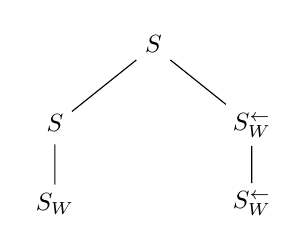
\begin{tikzpicture}
                [level/.style={sibling distance=25mm,
                               level distance=10mm}]
        \node [scale=0.9] (z){$S_{\tyr}$}
          child {node [scale=0.9] (a) {$S_{\tmr}$}
            child {node [scale=0.9] (a0) {$S_{\tmr W}$}}}
          child {node [scale=0.9] (b) {$S_W^{\leftarrow}$}
              child{node [scale=0.9] (d){$S_{\tyr W}^{\leftarrow}$}}};
%          \path (z) -- (a) node [midway] {$\leq$};
%          \path (z) -- (b) node [midway] {$\leq$};
              \end{tikzpicture}
  \end{minipage}  
  \caption{Dependencies between Context Schemas}
  \label{fig:ctxschema}
\end{wrapfigure}
In our proof development, we relied on different, but often related context schemas (invariants). 
Compared to many existing benchmarks, this challenge problem exhibits a particularly rich context structure. 
We describe the relationship between context schemas in Fig.~\ref{fig:ctxschema}. We can always weaken a context of schema $S_{\tyr}$ to any of the other schemas in the graph. Given our dependency graph of the different judgements (aka predicates), i.e.~$\tyr$, $\tmr$, etc., the graph also induces a strengthening relationship. We can always strengthen a context schema to pass it in place of a context that is higher in the hierarchy. 






%%% Local Variables:
%%% mode: latex
%%% TeX-master: "fscd17"
%%% End:
